\documentclass[oneside,a4paper,11pt]{report}
\usepackage{fullpage}
\usepackage{hhline}

\usepackage{../../info/packages}
\usepackage{../../info/nomenclature}
\usepackage{scalerel}

\title{Fluid Mechanics}
\author{Alejandro Campos}

\begin{document}
\maketitle
\tableofcontents

\chapter*{Preface}
\addcontentsline{toc}{chapter}{Preface}

%%%%%%%%%%%%%%%%%%%%%%%%%%%%%%%%%%%%%%%%%%%%%%%%%%%%%%%%%%%%%%%%%%%%%%%%%
\part{Inviscid Incompressible Flow}
%%%%%%%%%%%%%%%%%%%%%%%%%%%%%%%%%%%%%%%%%%%%%%%%%%%%%%%%%%%%%%%%%%%%%%%%%

%########################################################################	
\chapter{Inviscid solutions of the Navier Stokes Equations}
%########################################################################

%########################################################################
\chapter{Potential Flow}
%########################################################################
Velocity potential; Cauchy-Riemman eqs.; Laplace's eq.; Uniform, Source/Sink, Doublet and Vortex flows; Kutta-Joukowski Thm.; Cylinder flow.

%%%%%%%%%%%%%%%%%%%%%%%%%%%%%%%%%%%%%%%%%%%%%%%%%%%%%%%%%%%%%%%%%%%%%%%%%
\part{Viscous Flow}
%%%%%%%%%%%%%%%%%%%%%%%%%%%%%%%%%%%%%%%%%%%%%%%%%%%%%%%%%%%%%%%%%%%%%%%%%

%########################################################################
\chapter{Viscous solutions of the Navier Stokes Equations}
%########################################################################
Viscous effects include friction drag, flow separation(leading edge stall, trailing edge stall, thin airfoil stall), and viscous dissipation.

%------------------------------------------------------------------------
\section{Steady Parallel Flows}
%------------------------------------------------------------------------

%---------------------------------
\subsection{Couette flow} 
%---------------------------------

%---------------------------------
\subsection{Poiseuille flow (plane and circular)}
%---------------------------------

%---------------------------------
\subsection{Combined Couette and Poiseuille flow}
%---------------------------------

%------------------------------------------------------------------------
\section{Unsteady Parallel Flows}
%------------------------------------------------------------------------

%---------------------------------
\subsection{Stokes first problem}
%---------------------------------

%---------------------------------
\subsection{Stokes second problem}
%---------------------------------

%------------------------------------------------------------------------
\section{Lubrication Theory and Flow in thin structures}
%------------------------------------------------------------------------

%########################################################################
\chapter{Boundary Layers}
%########################################################################

%------------------------------------------------------------------------
\section{Introduction}
%------------------------------------------------------------------------

%---------------------------------
\subsection{Scaling of boundary layer thickness}
%---------------------------------

%---------------------------------
\subsection{B.L. eqs. as result of non-dimensionalization of NS eqs.}
%---------------------------------

%---------------------------------
\subsection{Displacement thickness (different interpretations), Momentum thickness}
%---------------------------------

%---------------------------------
\subsection{Iterative procedure for coupled viscous-inviscid solution.}
%---------------------------------

%------------------------------------------------------------------------
\section{Integral Methods}
%------------------------------------------------------------------------

%---------------------------------
\subsection{Von Karman Momentum Integral Equation}
%---------------------------------

%---------------------------------
\subsection{Pohlhausen}
%---------------------------------

%---------------------------------
\subsection{Thwaites}
%---------------------------------

%------------------------------------------------------------------------
\section{Exact Solutions}
%------------------------------------------------------------------------

%---------------------------------
\subsection{Blasius}
%---------------------------------

%---------------------------------
\subsection{Falkner Skan}
%---------------------------------

%%%%%%%%%%%%%%%%%%%%%%%%%%%%%%%%%%%%%%%%%%%%%%%%%%%%%%%%%%%%%%%%%%%%%%%%%
\appendix
%%%%%%%%%%%%%%%%%%%%%%%%%%%%%%%%%%%%%%%%%%%%%%%%%%%%%%%%%%%%%%%%%%%%%%%%%

%########################################################################
\chapter{Vectors in rotating reference frames}
%########################################################################

%------------------------------------------------------------------------
\section{Basic properties}
%------------------------------------------------------------------------

%--------------------------------------------
\subsection{Position}
%--------------------------------------------
Consider the Eucledian transformation
\begin{equation}
\label{eq:x_rot}
\tilde{x}^+_i(\tilde{t}) = Q_{ij}(\tilde{t}-c) x^+_j(\tilde{t}-c) + b_i(\tilde{t}-c) 
\end{equation}
where $x^+(t)$ is the Lagrangian position of a fluid particle, and $\tilde{x}^+(\tilde{t})$ is the Lagrangian position of the same particle but in a rotating reference frame. The transformation above amounts to a rotation of the reference frame determined by the orthogonal matrix $\mathbf{Q}(t)$, a translation of the reference frame determined by the vector $\mathbf{b}(t)$, and a translation in time given by $\tilde{t} = t + c$. 

%--------------------------------------------
\subsection{Velocity}
%--------------------------------------------
Since the velocity of a fluid particle is given by 
\begin{equation}
u^+_i(t) = \frac{d x^+_i(t)}{dt},
\end{equation}
the components of velocity in the non-inertial reference frame are defined as
\begin{equation}
\tilde{u}^+_i(\tilde{t}) = \frac{d \tilde{x}^+_i(\tilde{t})}{d \tilde{t}} .
\end{equation}
Thus, the relationship between the velocity components in the different reference frames is given by
\begin{align}
\label{eq:rot_vel_general}
\tilde{u}^+_i(\tilde{t}) &= \frac{d}{d\tilde{t}} [Q_{ij}(\tilde{t} - c) x^+_j(\tilde{t} - c) + b_i(\tilde{t} - c)] \nonumber \\
& = Q_{ij}(\tilde{t} - c) U^+_j(\tilde{t} - c) + \dot{Q}_{ij}(\tilde{t} - c) x^+_j(\tilde{t} - c) + \dot{b}_i(\tilde{t} - c).
\end{align}
If we assume there is no translation in space or time, the above reduces to
\begin{equation}
\label{eq:rot_vel_inter}
\tilde{u}^+_i = Q_{ij} u^+_j + \dot{Q}_{ij} x^+_j, 
\end{equation}
where each quantity above depends on time $t$. Multiplying by $Q^{-1}_{ki}$ we obtain
\begin{equation}
Q_{ik} \tilde{u}^+_i = u^+_k + Q_{ik}\dot{Q}_{ij}x^+_j.
\end{equation}
Noting that the tensor $Q_{ik} \dot{Q}_{ij}$ is antisymmetric, we obtain
\begin{equation}
\label{eq:rot_vel}
u^+_k = Q_{ik} \tilde{u}^+_i + Q_{ij}\dot{Q}_{ik}x^+_j.
\end{equation}

We now define the angular velocity tensor $\Omega_{ij}$ and the angular velocity vector $\Omega_i$ using the following relationship 
\begin{equation}
\label{eq:angular_definition}
\Omega_{ij} = \epsilon_{jik}\Omega_{k} = Q_{kj}\dot{Q}_{ki}.
\end{equation}
Thus (\ref{eq:rot_vel}) can be expressed in terms of the angular velocity tensor as
\begin{equation}
\label{eq:rot_vel_angular_tensor}
u^+_k = Q_{ik} \tilde{u}^+_i + \Omega_{kj}x^+_j,
\end{equation}
or in terms of the angular velocity vector as
\begin{equation}
\label{rot_vel_angular_vector}
u^+_k = Q_{ik} \tilde{u}^+_i + \epsilon_{jki}\Omega_ix^+_j.
\end{equation}

%--------------------------------------------
\subsection{Acceleration}
%--------------------------------------------
We assume again no translation in space or time. Taking the derivative of both sides of \cref{eq:rot_vel}
\begin{equation}
    \frac{du^+_k}{dt} = \dot{Q}_{ik} \tilde{u}^+_i + Q_{ik} \frac{d\tilde{u}^+_i}{dt} + \dot{Q}_{ik} \frac{dQ_{ij} x^+_j}{dt} + Q_{ij}\ddot{Q}_{ik} x^+_j.
\end{equation}
Using \cref{eq:x_rot} the above is re-written as
\begin{equation}
    \frac{du^+_k}{dt} = Q_{ik} \frac{d\tilde{u}^+_i}{dt} + 2 \dot{Q}_{ik} \tilde{u}^+_i + Q_{ij}\ddot{Q}_{ik} x^+_j.
\end{equation}
Re-writing the last term on the right-hand-side above leads to
\begin{equation}
    \frac{du^+_k}{dt} = Q_{ik} \frac{d\tilde{u}^+_i}{dt} + 2 \dot{Q}_{ik} \tilde{u}^+_i + \frac{d Q_{ij}\dot{Q}_{ik}}{dt} x^+_j - \dot{Q}_{ij} \dot{Q}_{ik} x^+_j.
\end{equation}
We now show that
\begin{align}
    \dot{Q}_{ij} \dot{Q}_{ik} & = \delta_{pi}\dot{Q}_{pj} \dot{Q}_{ik}  \nonumber \\
    & = Q_{pq}Q^{-1}_{qi} \dot{Q}_{pj} \dot{Q}_{ik}  \nonumber \\
    & = Q_{pq} \dot{Q}_{pj} Q_{iq} \dot{Q}_{ik} .
\end{align}
Thus, in terms of the angular velocity tensor, we have
\begin{equation}
    \frac{du^+_k}{dt} = Q_{ik} \frac{d\tilde{u}^+_i}{dt} + 2 \dot{Q}_{ik} \tilde{u}^+_i + \frac{d \Omega_{kj}}{dt} x^+_j - \Omega_{kq} \Omega_{jq} x^+_j.
\end{equation}
In terms of the angular velocity vector, the above becomes
\begin{equation}
    \frac{du^+_k}{dt} = Q_{ik} \frac{d\tilde{u}^+_i}{dt} + 2 \dot{Q}_{ik} \tilde{u}^+_i + \epsilon_{jki}\frac{d \Omega_{i}}{dt} x^+_j - \epsilon_{qki}\Omega_{i} \epsilon_{qjp}\Omega_{p} x^+_j,
\end{equation}
which, upon a simple re-arrangement of indices, gives
\begin{equation}
\label{eq:rot_acl_angular_vector}
    \frac{du^+_k}{dt} = Q_{ik} \frac{d\tilde{u}^+_i}{dt} + 2 \dot{Q}_{ik} \tilde{u}^+_i + \epsilon_{kij}\frac{d \Omega_{i}}{dt} x^+_j + \epsilon_{kiq}\Omega_{i} \epsilon_{qpj}\Omega_{p} x^+_j.
\end{equation}

%------------------------------------------------------------------------
\section{Unit vectors}
%------------------------------------------------------------------------
Let the orthogonal basis for the inertial reference frame be denoted by $\hat{a}^{(1)}$, $\hat{a}^{(2)}$, and $\hat{a}^{(3)}$, and the orthogonal basis for the rotating reference frame by $\hat{b}^{(1)}$, $\hat{b}^{(2)}$, and $\hat{b}^{(3)}$. We know that the unit vector $\hat{b}^{(i)}$ has components $\tilde{b}_j^{(i)}$ in the rotating reference frame, and components $b_j^{(i)}$ in the inertial reference frame. The vector is the same whether expressed in the rotating or inertial reference frames, that is
\begin{equation}
\tilde{b}_k^{(i)} \hat{b}^{(k)} = b_k^{(i)} \hat{a}^{(k)}
\end{equation}
Since $\tilde{b}_k^{(i)} = \delta_{ik}$, we rewrite the above as
\begin{equation}
\label{eq:unit_trans}
\hat{b}^{(i)} = b_k^{(i)} \hat{a}^{(k)} = Q_{jk} \tilde{b}_j^{(i)} \hat{a}^{(k)} = Q_{ik} \hat{a}^{(k)}.
\end{equation}
Doting both sides by $\hat{a}^{(j)}$ shows that 
\begin{equation}
Q_{ij} = \hat{a}^{(j)} \cdot \hat{b}^{(i)}.
\end{equation}

One can also multiply both sides of \cref{rot_vel_angular_vector} by $\hat{a}^{(k)}$ and use \cref{eq:unit_trans} to obtain
\begin{equation}
    \label{eq:uine_urot_temp}
u^+_k \hat{a}^{(k)} = \tilde{u}^+_i \hat{b}^{(i)} + \epsilon_{jki}\Omega_ix^+_j \hat{a}^{(k)}.
\end{equation}
If we introduce the following notation
\begin{align}
    \vec{u}^+_{ine} &= u^+_k \hat{a}^{(k)}, \\
    \vec{u}^+_{rot} &= \tilde{u}^+_i \hat{b}^{(i)}, \\
    \vec{\Omega} &= \Omega_i \hat{a}^{(i)}, \\
    \vec{x}^+ &= x_i^+ \hat{a}^{(i)}.
\end{align}
then the \cref{eq:uine_urot_temp} is writen as 
\begin{equation}
\label{uine_urot}
\vec{u}^+_{ine}  = \vec{u}^+_{rot}  + \vec{\Omega} \times \vec{x}^+.
\end{equation}
Similarly, multiplying both sides of \cref{eq:rot_acl_angular_vector} gives
\begin{equation}
\label{eq:aine_arot_inter}
    \frac{du^+_k}{dt} \hat{a}^{(k)} = \frac{d\tilde{u}^+_i}{dt}\hat{b}^{(i)} + 2 \dot{Q}_{ik} \tilde{u}^+_i \hat{a}^{(k)} + \epsilon_{kij}\frac{d \Omega_{i}}{dt} x^+_j \hat{a}^{(k)} + \epsilon_{kiq}\Omega_{i} \epsilon_{qpj}\Omega_{p} x^+_j \hat{a}^{(k)}.
\end{equation}
Using \cref{eq:angular_definition} one can show that $\dot{Q}_{ik} = \epsilon_{pjk} \Omega_p Q_{ij}$. Thus, the second term on the left-hand-side above can be written as
\begin{align}
    2 \dot{Q}_{ik} \tilde{u}^+_i \hat{a}^{(k)} &= 2 \epsilon_{pjk} \Omega_p Q_{ij} \tilde{u}^+_i \hat{a}^{(k)} \nonumber \\
    &= 2 \Omega_p Q_{ij} \tilde{u}^+_i \hat{a}^{(p)} \times \hat{a}^{(j)} \nonumber \\
    &= 2 \Omega_p \hat{a}^{(p)} \times \tilde{u}^+_i \hat{b}^{(i)}.
\end{align}
Therefore, in vector notation \cref{eq:aine_arot_inter} becomes
\begin{equation}
    \label{eq:aine_arot}
    \vec{a}^+_{ine} = \vec{a}^+_{rot} + 2 \vec{\Omega} \times \vec{u}^+_{rot} + \dot{\vec{\Omega}} \times \vec{x}^+ + \vec{\Omega} \times (\vec{\Omega} \times \vec{x}^+),
\end{equation}
where $\vec{a}^+_{ine} = \frac{du^+_k}{dt} \hat{a}^{(k)}$, $\vec{a}^+_{rot} = \frac{d\tilde{u}^+_i}{dt}\hat{b}^{(i)}$, and $\dot{\vec{\Omega}} = \frac{d\Omega_i}{dt} \hat{a}^{(i)}$.

%------------------------------------------------------------------------
\section{Eulerian variables}
%------------------------------------------------------------------------
We now introduce the Eulerian counterpart to the Lagrangian variables. In the inertial reference frame these are $\rho(t,\xvec)$, $u_i(t,\xvec)$, and $p(t,\xvec)$. They are defined by the following expressions
\begin{align}
    \rho^+ &= \rho(t,\xvec^+) \\
    u_i^+ &= u_i(t,\xvec^+) \\
    p^+ &= p(t,\xvec^+).
\end{align}
Similarly for the rotating reference frame, we have $\tilde{\rho}(t,\tilde{\xvec})$, $\tilde{u}_i(t,\tilde{\xvec})$, and $\tilde{p}(t,\tilde{\xvec})$. These are defined by
\begin{align}
    \tilde{\rho}^+ &= \tilde{\rho}(t,\tilde{\xvec}^+) \\
    \tilde{u}_i^+ &= \tilde{u}_i(t,\tilde{\xvec}^+) \\
    \tilde{p}^+ &= \tilde{p}(t,\tilde{\xvec}^+).
\end{align}
We now use the transformation rules for the Lagrangian variables to derive the transformation rules for the Eulerian variables. The transformation rules for the Lagrangian variables are
\begin{align}
    \rho^+ &= \tilde{\rho}^+ \\
    u_k^+ &= Q_{ik} \tilde{u}_i^+ + Q_{ij} \dot{Q}_{ik} x_j^+ \\
    p^+ &= \tilde{p}^+.
\end{align}
The second equation above is the previously derived \cref{eq:rot_vel}. Using the definition of the Eulerian variables, the above is re-written as
\begin{align}
    \rho(t,\xvec^+) &= \tilde{\rho}(t,\tilde{\xvec}^+) \label{eq:eul_rho_temp} \\
    u_i(t,\xvec^+) &= Q_{ik} \tilde{u}_i(t,\tilde{\xvec}^+)  + Q_{ij} \dot{Q}_{ik} x_j^+ \label{eq:eul_vel_temp}\\
    p(t,\xvec^+) &= \tilde{p}(t,\tilde{\xvec}^+). \label{eq:pres_temp}
\end{align}
Using \cref{eq:x_rot}, we get
\begin{align}
    \rho(t,\xvec^+) &= \tilde{\rho}(t,\Qvec \xvec^+) \\
    u_i(t,\xvec^+) &= Q_{ik} \tilde{u}_i(t,\Qvec \xvec^+)  + Q_{ij} \dot{Q}_{ik} x_j^+ \\
    p(t,\xvec^+) &= \tilde{p}(t,\Qvec \xvec^+)+.
\end{align}
Since the above holds for any $\xvec^+$, we finally re-write it as
\begin{align}
    \rho(t,\xvec) &= \tilde{\rho}(t,\Qvec \xvec) \label{eq:eul_rho_trans}\\
    u_i(t,\xvec) &= Q_{ik} \tilde{u}_i(t,\Qvec \xvec)  + Q_{ij} \dot{Q}_{ik} x_j \label{eq:eul_vel_trans}\\
    p(t,\xvec) &= \tilde{p}(t,\Qvec \xvec). \label{eq:eul_pres_trans}
\end{align}

%------------------------------------------------------------------------
\section{Rotating Navier-Stokes equations}
%------------------------------------------------------------------------
We first obtain a few set of relationships that will later be used in deriving the rotating Navier-Stokes equations. Taking the derivative of \cref{eq:eul_pres_trans} gives
\begin{align}
    \frac{\partial p(t,\xvec)}{\partial x_i} &= \frac{ \partial \tilde{p}(t,\Qvec \xvec)}{\partial x_i} \nonumber \\
    &= \frac{\partial}{\partial x_i} \tilde{p}(t,Q_{1j}x_j, Q_{2j}x_j, Q_{3j} x_3) \nonumber \\
    &= \frac{\partial Q_{1j}x_j}{\partial x_i} \left [ \frac{\partial \tilde{p}(t,\tilde{\xvec})}{\partial \tilde{x}_1} \right]_{ \tilde{\xvec} = \Qvec \xvec} + \frac{\partial Q_{2j}x_j}{\partial x_i} \left [ \frac{\partial \tilde{p}(t,\tilde{\xvec})}{\partial \tilde{x}_2} \right ]_{\tilde{\xvec} = \Qvec \xvec} + \frac{\partial Q_{3j}x_j}{\partial x_i} \left [ \frac{\partial \tilde{p}(t,\tilde{\xvec})}{\partial \tilde{x}_3} \right ]_{\tilde{\xvec} = \Qvec \xvec} \nonumber \\
    &= Q_{ji} \left [ \frac{\partial \tilde{p}(t,\tilde{\xvec})}{\partial \tilde{x}_j} \right ]_{\tilde{\xvec} = \Qvec \xvec}
\end{align}
If we evaluate the above at $\xvec = \xvec^+$, we get
\begin{equation}
    \left [ \frac{\partial p(t,\xvec)}{\partial x_i} \right]_{\xvec = \xvec^+} = Q_{ji} \left [ \frac{\partial \tilde{p}(t,\tilde{\xvec})}{\partial \tilde{x}_j} \right]_{\tilde{\xvec} = \tilde{\xvec}^+}.
\end{equation}
Multiplying both sides by $\hat{a}^{(i)}$ gives
\begin{equation}
\label{eq:ns_pressure_rot_transform}
    \left [ \frac{\partial p(t,\xvec)}{\partial x_i} \right]_{\xvec = \xvec^+} \hat{a}^{(i)} = \left [ \frac{\partial \tilde{p}(t,\tilde{\xvec})}{\partial \tilde{x}_j} \right]_{\tilde{\xvec} = \tilde{\xvec}^+} \hat{b}^{(j)}.
\end{equation}
For the shear-stress tensor, we have
\begin{equation}
    \label{eq:ns_shear_stress_rot_transform}
    \left [ \frac{\partial \tau_{ij}(t,\xvec)}{\partial x_j} \right]_{\xvec = \xvec^+} \hat{a}^{(i)} = \left [ \frac{\partial \tilde{\tau}_{ij}(t,\tilde{\xvec})}{\partial \tilde{x}_j} \right]_{\tilde{\xvec} = \tilde{\xvec}^+} \hat{b}^{(i)}.
\end{equation}
We also use \cref{eq:aine_arot} to write
\begin{align}
    \frac{du_i^+}{dt} \hat{a}^{(i)} &= \frac{d\tilde{u}_i^+}{dt} \hat{b}^{(i)} + 2 \vec{\Omega} \times \left ( \tilde{u}_i^+ \hat{b}^{(i)} \right ) + \dot{\vec{\Omega}} \times \vec{x}^+ + \vec{\Omega} \times \left ( \vec{\Omega} \times \vec{x}^+ \right ) \nonumber \\
    &= \frac{d\tilde{u}_i^+}{dt} \hat{b}^{(i)} + 2 \vec{\Omega} \times \left ( \tilde{u}_i^+ \hat{b}^{(i)} \right ) + \dot{\vec{\Omega}} \times \left ( \tilde{x}_i^+ \hat{b}^{(i)}\right ) + \vec{\Omega} \times \left [ \vec{\Omega} \times \left ( \tilde{x}_i^+ \hat{b}^{(i)}\right ) \right ]
\end{align}
Expressing the above in terms of Eulerian quantities gives
\begin{multline}
    \label{eq:aine_arot_eulerian}
    \left [ \frac{\partial u_i(t,\xvec)}{\partial t} + u_j(t,\xvec) \frac{\partial u_i(t,\xvec)}{\partial x_j} \right ]_{\xvec = \xvec^+} \hat{a}^{(i)} = \left [ \frac{\partial \tilde{u}_i(t,\tilde{\xvec})}{\partial t} + \tilde{u}_j(t,\tilde{\xvec}) \frac{\partial \tilde{u}_i(t,\tilde{\xvec})}{\partial \tilde{x}_j} \right ]_{\tilde{\xvec} = \tilde{\xvec}^+} \hat{b}^{(i)} \\
    + 2 \vec{\Omega} \times \left \{ \left [\tilde{u}_i(t,\tilde{\xvec}) \right ]_{\tilde{\xvec} = \tilde{\xvec}^+} \hat{b}^{(i)} \right \} + \dot{\vec{\Omega}} \times \left [ \left ( \tilde{x}_i \right)_{\tilde{\xvec} = \tilde{\xvec}^+} \hat{b}^{(i)}\right ] + \vec{\Omega} \times \left \{ \vec{\Omega} \times \left [ \left ( \tilde{x}_i \right )_{\tilde{\xvec} = \tilde{\xvec}^+} \hat{b}^{(i)}\right ] \right \}
\end{multline}

The conservation of momentum equation is given by
\begin{equation}
    \rho(t,\xvec) \left [\frac{\partial u_i(t,\xvec)}{\partial t} + u_j(t,\xvec) \frac{\partial u_i(t,\xvec)}{\partial x_j} \right ] = -\frac{\partial p(t,\xvec)}{\partial x_i} + \frac{\partial \tau_{ij}(t,\xvec)}{\partial x_j}.
\end{equation}
Evaluating the above at $\xvec = \xvec^+$ can be written as
\begin{equation}
    \rho(t,\xvec^+) \left [\frac{\partial u_i(t,\xvec)}{\partial t} + u_j(t,\xvec) \frac{\partial u_i(t,\xvec)}{\partial x_j} \right ]_{\xvec = \xvec^+} = -\left [ \frac{\partial p(t,\xvec)}{\partial x_i} \right]_{\xvec = \xvec^+} + \left [ \frac{\partial \tau_{ij}(t,\xvec)}{\partial x_j} \right ]_{\xvec = \xvec^+}.
\end{equation}
Multiplying both sides by $\hat{a}^{(i)}$ gives
\begin{multline}
    \rho(t,\xvec^+) \left [\frac{\partial u_i(t,\xvec)}{\partial t} + u_j(t,\xvec) \frac{\partial u_i(t,\xvec)}{\partial x_j} \right ]_{\xvec = \xvec^+} \hat{a}^{(i)} \\
    = -\left [ \frac{\partial p(t,\xvec)}{\partial x_i} \right]_{\xvec = \xvec^+} \hat{a}^{(i)} + \left [ \frac{\partial \tau_{ij}(t,\xvec)}{\partial x_j} \right ]_{\xvec = \xvec^+} \hat{a}^{(i)}.
\end{multline}
Using \cref{eq:eul_rho_temp,eq:ns_pressure_rot_transform,eq:ns_shear_stress_rot_transform} gives
\begin{multline}
    \left [ \tilde{\rho}(t,\tilde{\xvec}) \right]_{\tilde{\xvec} = \tilde{\xvec}^+} \left [\frac{\partial u_i(t,\xvec)}{\partial t} + u_j(t,\xvec) \frac{\partial u_i(t,\xvec)}{\partial x_j} \right ]_{\xvec = \xvec^+} \hat{a}^{(i)} \\
    = -\left [ \frac{\partial \tilde{p}(t,\tilde{\xvec})}{\partial \tilde{x}_i} \right]_{\tilde{\xvec} = \tilde{\xvec}^+} \hat{b}^{(i)} + \left [ \frac{\partial \tilde{\tau}_{ij}(t,\tilde{\xvec})}{\partial \tilde{x}_j} \right ]_{\tilde{\xvec} = \tilde{\xvec}^+} \hat{b}^{(i)}.
\end{multline}
Using \cref{eq:aine_arot_eulerian} we obtain
\begin{multline}
    \left [ \tilde{\rho}(t,\tilde{\xvec}) \right]_{\tilde{\xvec} = \tilde{\xvec}^+} \left ( \left [ \frac{\partial \tilde{u}_i(t,\tilde{\xvec})}{\partial t} + \tilde{u}_j(t,\tilde{\xvec}) \frac{\partial \tilde{u}_i(t,\tilde{\xvec})}{\partial \tilde{x}_j} \right ]_{\tilde{\xvec} = \tilde{\xvec}^+} \hat{b}^{(i)} + 2 \vec{\Omega} \times \left \{ \left [\tilde{u}_i(t,\tilde{\xvec}) \right ]_{\tilde{\xvec} = \tilde{\xvec}^+} \hat{b}^{(i)} \right \} \right . \\
    \left . + \dot{\vec{\Omega}} \times \left [ \left ( \tilde{x}_i \right)_{\tilde{\xvec} = \tilde{\xvec}^+} \hat{b}^{(i)}\right ] + \vec{\Omega} \times \left \{ \vec{\Omega} \times \left [ \left ( \tilde{x}_i \right )_{\tilde{\xvec} = \tilde{\xvec}^+} \hat{b}^{(i)}\right ] \right \} \right ) = -\left [ \frac{\partial \tilde{p}(t,\tilde{\xvec})}{\partial \tilde{x}_i} \right]_{\tilde{\xvec} = \tilde{\xvec}^+} \hat{b}^{(i)} + \left [ \frac{\partial \tilde{\tau}_{ij}(t,\tilde{\xvec})}{\partial \tilde{x}_j} \right ]_{\tilde{\xvec} = \tilde{\xvec}^+} \hat{b}^{(i)}.
\end{multline}
Finally, since this holds for any $\tilde{\xvec}^+$, we get
\begin{multline}
    \tilde{\rho}(t,\tilde{\xvec}) \left \{ \left [ \frac{\partial \tilde{u}_i(t,\tilde{\xvec})}{\partial t} + \tilde{u}_j(t,\tilde{\xvec}) \frac{\partial \tilde{u}_i(t,\tilde{\xvec})}{\partial \tilde{x}_j} \right ] \hat{b}^{(i)} + 2 \vec{\Omega} \times \left [ \tilde{u}_i(t,\tilde{\xvec}) \hat{b}^{(i)} \right ] \right . \\
    \left . + \dot{\vec{\Omega}} \times \left ( \tilde{x}_i \hat{b}^{(i)}\right ) + \vec{\Omega} \times \left [ \vec{\Omega} \times \left ( \tilde{x}_i \hat{b}^{(i)} \right ) \right ] \right \} = -\frac{\partial \tilde{p}(t,\tilde{\xvec})}{\partial \tilde{x}_i} \hat{b}^{(i)} + \frac{\partial \tilde{\tau}_{ij}(t,\tilde{\xvec})}{\partial \tilde{x}_j} \hat{b}^{(i)}.
\end{multline}

%########################################################################
\chapter{Multi-component fluid flows in thermochemical nonequilibrium}
%########################################################################
In this chapter we describe the governing equations for a system of species in thermochemical nonequilibrium. The total number of molecular species is $nms$ and the total number of species (atomic + molecular) is $ns$.
%------------------------------------------------------------------------
\section{Conservation equations}
%------------------------------------------------------------------------
The conservation equations that govern the dynamics of a compressible gas in thermochemical nonequilibrium are the following:
\begin{equation}
\frac{\partial \rho}{\partial t} + \frac{\partial \rho u_i}{\partial x_i} = 0
\end{equation}
\begin{equation}
\frac{\partial \rho u_i}{\partial t} + \frac{\partial \rho u_i u_j}{\partial x_j} = - \frac{\partial p}{\partial x_i} + \frac{\partial t_{ij}}{\partial x_j} + \rho f_i
\end{equation}
\begin{equation}
\frac{\partial \rho E}{\partial t} + \frac{\partial}{\partial x_i} \left [ \rho \left ( E + \frac{p}{\rho} \right ) u_i \right ] = \frac{\partial u_i t_{ij}}{\partial x_j} + \rho f_i u_i -  \frac{\partial q_i}{\partial x_i}
\end{equation}
\begin{equation}
\frac{\partial \rho e^{(v)}}{\partial t} + \frac{\partial \rho e^{(v)} u_i}{\partial x_i}  = -  \frac{\partial q_i^{(v)}}{\partial x_i} + Q^{(v)}
\end{equation}
\begin{equation}
\frac{\partial\rho Y_\alpha}{\partial t}+\frac{\partial \rho Y_\alpha u_i}{\partial x_i} = -\frac{\partial J_{\alpha,i}}{\partial x_i} + w_\alpha \quad \alpha \in [1,ns]
\end{equation}

%------------------------------------------------------------------------
\section{Transport models}
%------------------------------------------------------------------------

%------------------------------------------ 
\subsection{Shear stress, heat fluxes, and diffusive flux}
%------------------------------------------ 
The shear stress, heat flux, and diffusive flux are given by
\begin{equation}
t_{ij} = 2\mu S_{ij}^*
\end{equation}
\begin{equation}
q_i = -\kappa^{(t,r)} \frac{\partial T^{(t,r)}}{\partial x_i} - \kappa^{(v)} \frac{\partial T^{(v)}}{\partial x_i}  + \sum_{\alpha=1}^{nms} h_\alpha J_{\alpha,i}
\end{equation}
\begin{equation}
q_i^{(v)} = -\kappa^{(v)} \frac{\partial T^{(v)}}{\partial x_i} + \sum_{\alpha = 1}^{nms} e_\alpha^{(v)} J_{\alpha,i}
\end{equation}
\begin{equation}
J_{\alpha,i} = -\rho \left ( D_\alpha \frac{\partial Y_\alpha}{\partial x_i} - Y_\alpha \sum_\beta^{ns} D_\beta \frac{\partial Y_\beta}{\partial x_i} \right ) \quad \alpha \in [1,ns]
\end{equation}

%------------------------------------------ 
\subsection{Transport coefficients}
%------------------------------------------ 
The transport coefficients $\mu$, $\kappa^{(t,r)}$, $\kappa^{(v)}$, and $D_\alpha$ required by the models above still need to be specified. There are a wide variety of models for these transport coefficients, and a few of these are detailed below. 

The species viscosity $\mu_\alpha$ is computed using a Blottner curve fit \cite{blottner1971},
\begin{equation}
    \mu_\alpha = 0.1 \exp \left [ \left ( A_\alpha^\mu \ln T^{(t,r)} + B_\alpha^\mu \right ) \ln T^{(t,r)} + C_\alpha^\mu \right ]
\end{equation}
The coefficients $A_\alpha^\mu$, $B_\alpha^\mu$, and $C_\alpha^\mu$ are listed in \cite{blottner1971}. The species translational-rotational thermal conductivity is computed using the Eucken relation
\begin{equation}
\kappa_\alpha = \mu_\alpha \left ( \frac{f}{2} + 2.25 \right ) R,
\end{equation}
where $f$ is the number of translational and rotational degrees of freedom (3 for monatomic gas and 5 for diatomic gas). The species vibrational thermal conductivity is computed as follows
\begin{equation}
    \kappa_\alpha^{(v)} = \mu_\alpha C_{v,\alpha}^{(v)},
\end{equation}
where $C_{v,\alpha}^{(v)}$ is the heat capacity at constant volume for the vibrational energy of a given species $\alpha$ (i.e. $C_{v,\alpha}^{(v)} = d e_\alpha^{(v)} / d T^{(v)}$).
\begin{equation}
D_\alpha = \frac{\mu}{\rho Sc_\alpha} \quad \alpha \in [1,ns]
\end{equation}

The viscosity $\mu$ for the whole mixture is obtained from the viscosity of each species $\mu_\alpha$ using the Wilke mixing rule \cite{wilke1950}
\begin{equation}
\mu = \sum_{\alpha = 1}^{ns} \frac{X_\alpha \mu_\alpha}{\phi_\alpha},
\end{equation}
where $\phi_\alpha$ is computed using
\begin{equation}
\label{eq:wilke_mixing_phi}
    \phi_\alpha = \sum_{\beta = 1}^{ns} X_\beta \frac{ \left [ 1 + \left ( \frac{\mu_\alpha}{\mu_\beta} \right )^{1/2} \left ( \frac{M_\beta}{M_\alpha} \right)^{1/4} \right]^2}{ \left [ 8 \left ( 1 + \frac{M_\alpha}{M_\beta} \right ) \right ]^{1/2} }.
\end{equation}
Note that the equation for the Wilke mixing rule given in \cite{palmer2003} differs from the above since it doesn't include the $X_\beta$ shown in \cref{eq:wilke_mixing_phi}. 

%------------------------------------------------------------------------
\section{Equation of state}
%------------------------------------------------------------------------

%------------------------------------------ 
\subsection{Perfect gas}
%------------------------------------------ 
\begin{equation}
p = \rho R T 
\end{equation}
\begin{equation}
R = \frac{R_u}{M}
\end{equation}
\begin{equation}
\frac{1}{M} = \sum_\alpha \frac{Y_\alpha}{M_\alpha}
\end{equation}

%------------------------------------------ 
\subsection{Ideal gas}
%------------------------------------------

%------------------------------------------------------------------------
\section{Thermal nonequilibrium}
%------------------------------------------------------------------------

%------------------------------------------ 
\subsection{Energy definitions}
%------------------------------------------ 
The total energy of the system $E$ is expressed as follows
\begin{equation}
E = e^{(t)} + e^{(r)} + e^{(v)} + e^{(el)} + e^{(e)} + \sum_{\alpha =1}^{ns} Y_\alpha h_\alpha^o + \frac{1}{2}u_i u_i .
\end{equation}
In the above, $e^{(t)}$ is the translation energy, $e^{(v)}$ the vibration energy, $e^{(el)}$ the electronic energy, and $e^{(e)}$ the electron energy. $h_\alpha^o$ denotes the heat of formation for each species. Each of the energies can be computed in terms of its single-species counterpart, as follows
\begin{align}
e^{(t)} &= \sum_{\alpha =1}^{ns} Y_\alpha e^{(t)}_\alpha \\
e^{(r)} & = \sum_{\alpha = 1}^{nms} Y_\alpha e^{(r)}_\alpha \\
e^{(v)} & = \sum_{\alpha =1}^{nms} Y_\alpha e^{(v)}_\alpha \\
e^{(el)} & = \sum_{\alpha =1}^{nms} Y_\alpha e^{(el)}_\alpha.
\end{align}
The translational energy for each single species is computed using
\begin{equation}
e^{(t)}_\alpha = \frac{3}{2} R_\alpha T^{(t,r)} \quad \alpha \in [1,ns].
\end{equation}
The rotational energy for each single species is computed using
\begin{equation}
e^{(r)}_\alpha = R_\alpha T^{(t,r)} \quad \alpha \in [1,nms].
\end{equation}
The vibrational energy for each single species is computed using
\begin{equation}
e^{(v)}_\alpha = \sum_{\beta = 1}^{nvm} g_{\alpha,\beta}R_\alpha \frac{\theta^{(v)}_{\alpha,\beta}}{\exp \left ( \theta^{(v)}_{\alpha,\beta} / T^{(v)} \right ) - 1} \quad \alpha \in [1,nms].
\end{equation}
In the above, $nvm$ is the number of vibrational modes, $g_{\alpha,\beta}$ is the degeneracy of each vibrational mode, and $\theta^{(v)}_{\alpha,\beta}$ is the characteristic vibrational temperature of each vibrational mode. The characteristic temperatures for $N_2$, $O_2$, and $NO$ can be found in \cite{park1990}, for $C_3$ in \cite{dolton1968}, and for $CO_2$, $C_2$, $CO$, and $CN$ in \cite{mcbride1963}. For our current purposes, both the electronic and electron energy are not accounted for, i.e.,
\begin{equation}
e_{el,\alpha} = 0  \quad \alpha \in [1,nms],
\end{equation}
\begin{equation}
e_e = 0.
\end{equation}

%------------------------------------------ 
\subsection{Temperature equilibration}
%------------------------------------------ 
The source term for the vibrational energy is 
\begin{equation}
Q^{(v)} = \sum_{\alpha = 1}^{nms} Q^{(t,r-v)}_\alpha + w_\alpha e^{(v)}_\alpha.
\end{equation}
In the above, $Q_{t-v,\alpha}$ represents the exchange of energy between translation-rotation and vibration energies. It is modeled using the Landau-Teller formulation
\begin{equation}
Q^{(t,r-v)}_\alpha = \rho Y_\alpha \frac{ e^{(v)}_\alpha (T^{(t,r)}) - e^{(v)}_\alpha(T^{(v)}) }{ \left < \tau_\alpha \right > + \tau^{(c)}_\alpha } \quad \alpha \in [1,nms]. 
\end{equation}
The Landau-Teller relaxation time given by \cite{lee1985} is
\begin{equation}
\left < \tau_\alpha \right > = \frac{ \sum_{\beta = 1}^{ns} X_\beta}{ \sum_{\beta = 1}^{ns} X_\beta / \tau_{\alpha,\beta}}.
\end{equation}
The expression used for $\tau_{\alpha,\beta}$ is that from \cite{millikan1963}
\begin{equation}
\tau_{\alpha,\beta} = \frac{1}{p} \exp \left [ A_{\alpha,\beta} \left ( \left. T^{(t,r)} \right .^{-1/3} - B_{\alpha,\beta} \right ) - 18.42 \right ], \quad p \text{ in atm}
\end{equation}
\begin{equation}
A_{\alpha,\beta} = 1.16 \times 10^{-3} \mu_{\alpha,\beta}^{1/2} \left .\theta_{\alpha,1}^{(v)} \right.^{4/3}
\end{equation}
\begin{equation}
B_{\alpha,\beta} = 0.015 \mu_{\alpha,\beta}^{1/4}
\end{equation}
\begin{equation}
\mu_{\alpha,\beta} = \frac{M_{\alpha} M_{\beta}}{ M_\alpha + M_\beta} \times 1000
\end{equation}
The relaxation time correction is that defined in \cite{park1990}, which is given by
\begin{equation}
\tau^{(c)}_\alpha = \frac{1}{C_\alpha \sigma_v n}
\end{equation}
In the above, $n$ is the mixture particle density, and $C_\alpha$ and $\sigma_v$ are computed as follows
\begin{equation}
C_\alpha = \sqrt{ \frac{8}{\pi} R_\alpha T^{(t,r)}},
\end{equation}
\begin{equation}
\sigma_v = 3 \times 10^{-21} \left ( \frac{50000}{T^{(t,r)}} \right )^2.
\end{equation}


%------------------------------------------------------------------------
\section{Chemical nonequilibrium}
%------------------------------------------------------------------------
The reaction rate for each species $\alpha$ is given by
\begin{equation}
w_\alpha = \sum_{\beta = 1}^{nr} w_{\alpha, \beta},
\end{equation}
where $w_{\alpha, \beta}$ is the reaction rate for species $\alpha$ due only to the chemical reaction $\beta$, and $nr$ is the total number of reactions. The reaction rates $w_{\alpha,\beta}$ are usually expressed in terms of the progress rate $\mathcal{Q}_\beta$ as follows
\begin{equation}
w_{\alpha,\beta} = M_\alpha \nu_{\alpha, \beta} \mathcal{Q}_\beta.
\end{equation}
In the above, $\nu_{\alpha,\beta} = \nu_{\alpha,\beta}'' - \nu_{\alpha,\beta}'$, where $\nu_{\alpha,\beta}'$ and $\nu_{\alpha,\beta}''$ are the molar stoichiometric coefficients on the left and right hand side of a reaction, respectively.

The progress rate $\mathcal{Q}_\beta$ of reaction $\beta$ is given by
\begin{equation}
\mathcal{Q}_\beta = K^{(f)}_\beta \prod_{\alpha = 1}^{ns} [ X_\alpha ]^{\nu_{\alpha, \beta}'} - K^{(b)}_\beta \prod_{\alpha = 1}^{ns} [X_\alpha]^{\nu_{\alpha, \beta}''},
\end{equation}
where $K^{(f)}_\beta$ and $K^{(b)}_\beta$ are the forward and backward rate constants, and $[X_\alpha]$ is the molar concentration $([X_\alpha] = \rho Y_\alpha / M_\alpha)$. The forward rate constant is computed using the empirical Arrhenius law
\begin{equation}
K^{(f)}_\beta = A_\beta \left ( T^{(c)} \right)^{\eta_\beta} \exp \left ( -\frac{\theta_\beta}{T^{(c)}} \right ).
\end{equation}
For the above, $A_\beta$ is the pre-exponential factor, $\eta_\beta$ is the temperature exponent, and $\theta_\beta$ is the activation temperature---these are obtained from tables for each reaction $\beta$, and can be found, for example, in \cite{park1993}. $T^{(c)}$ is the controlling temperature, which depends on the type of reaction under consideration. For example, for dissociation reactions $T^{(c)}$ is typically of the form $T^{(c)} = \sqrt{ T^{(t,r)} T^{(v)}}$, whereas for exchange reactions $T^{(c)} = T^{(t,r)}$. The backward rate constant $K^{(b)}_\beta$ is often computed from the forward rate constant using $K^{(b)}_\beta = K^{(f)}_\beta / K_{eq}$. Multiple forms for $K_{eq}$ are available, see \cite{poinsot2012,knisely2018}.

%------------------------------------------------------------------------
\section{Additional relations}
%------------------------------------------------------------------------
\begin{equation}
    S^*_{ij} = \frac{1}{2} \left ( \frac{\partial u_i}{\partial x_j} + \frac{\partial u_j}{\partial x_i} \right ) - \frac{1}{3} \frac{\partial u_k}{\partial x_k} \delta_{ij}
\end{equation}

%########################################################################
\chapter{Aerodynamics}
%########################################################################
To compute total forces and moments on an aerodynamic body, integration over its surface is performed. Thus, at each point of the surface $s$, the contribution to the total force or moment due to the local stress vector $\Tvec$ is added. That is,
\begin{itemize}
    \item total force vector
    \begin{equation}
        \Fvec = \int_s \Tvec \, ds,
    \end{equation}
    \item total moment about the leading edge 
    \begin{equation}
        \Mvec_{le} = \int_s \rvec \times \Tvec \, ds.
    \end{equation}
\end{itemize}
In the above, $\rvec$ points from the leading edge to the point on the surface at which we are evaluating the stress vector. Note that the stress vector is given by $\Tvec = \boldsymbol{\sigma} \cdot \nvec$ (where $\nvec$ is the normal to the surface) and that the stress tensor is given by $\boldsymbol{\sigma} = -p \Ivec + \tvec$. The moment about an arbitrary point, rather than the leading edge, can be written as
\begin{equation}
\label{eq:moment_shift}
    \Mvec_{ap} = \int_s (\rvec - \rvec_{ap} ) \times \Tvec \, ds = \Mvec_{le} - \rvec_{ap} \times \int_s  \Tvec \, ds,
\end{equation}
where $\rvec_{ap}$ is the vector pointing from the leading edge to the arbitrary point. 

\begin{figure}[ht]
   \centering
   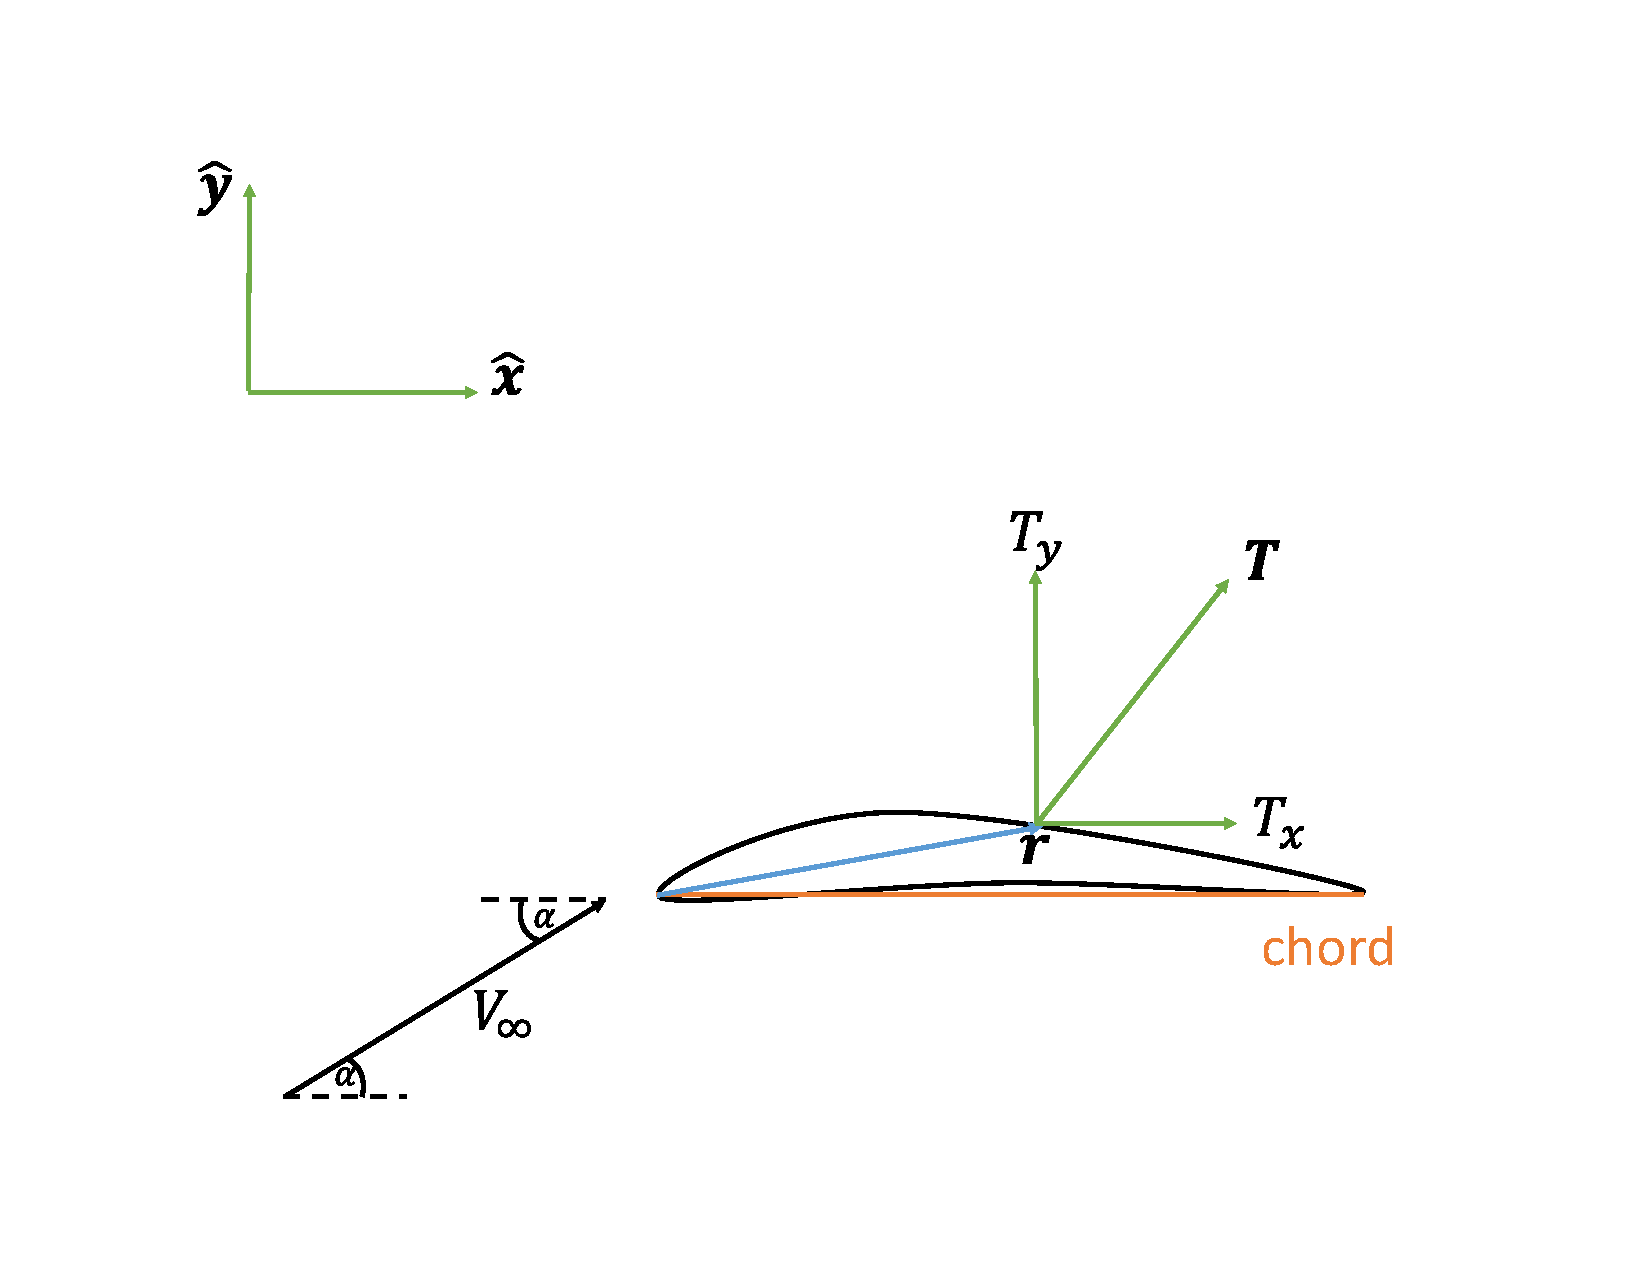
\includegraphics[width=0.8\textwidth]{../../images/airfoil.pdf}
   \caption{Coordinate system and representative forces on an airfoil.}
   \label{fig:airfoil}
\end{figure}

Consider the two dimensional case, as shown in \cref{fig:airfoil}. We label the normal force as
\begin{equation}
    F_N = \int_s T_y \, ds,
\end{equation}
and the tangential force as
\begin{equation}
    F_T = \int_s T_x \, ds.
\end{equation}
The moment about the leading edge, which points only along the $z$ direction only, can be written as
\begin{equation}
    M_{le} = \int_s (x \hat{\xvec} + y \hat{\yvec} ) \times (T_x \hat{\xvec} + T_y \hat{\yvec}) \, ds = \int_s x T_y - y T_x \, ds.
\end{equation}
Note that, for this convention, a positive moment decreases the angle of attach, and a negative moment increases the angle of attack---this is the opposite convention of Anderson. If we choose to compute the moment along an arbitrary point on the chord of the body, then \Cref{eq:moment_shift} becomes
\begin{equation}
    M_{ap} = M_{le} - x_{ap} F_N.
\end{equation}
The center of pressure is defined as the point along the chord for which the total moment becomes zero. Thus, it's location $x_{cp}$ is given by
\begin{equation}
    x_{cp} = \frac{M_{le}}{F_N}.
\end{equation}

The drag is defined as the force aligned with the free stream velocity, whereas the lift is the force normal to the free stream velocity. For 2D geometries, the direction of lift is well defined, whereas for 3D geometries, we pick the component of the force normal to the free stream velocity that points in the ``up'' direction. In terms for the normal and and tangential force, the lift and drag for a 2D geometry are given by
\begin{equation}
    \begin{bmatrix} L \\ D \end{bmatrix} = 
    \begin{bmatrix} \cos \alpha & \sin \alpha \\ -\sin \alpha & \cos \alpha \end{bmatrix} \begin{bmatrix} A \\ N \end{bmatrix}.
\end{equation}
Given the aerodynamics pressure
\begin{equation}
    q_\infty = \frac{1}{2} \rho_\infty V^2_\infty,
\end{equation}
a reference surface $S$, and a reference length $l$, the lift coefficient is given by
\begin{equation}
    C_L = \frac{L}{q_\infty S},
\end{equation}
the drag coefficient by
\begin{equation}
    C_D = \frac{L}{q_\infty S},
\end{equation}
and the moment coefficient by
\begin{equation}
    C_M = \frac{M}{q_\infty Sl}.
\end{equation}

%########################################################################
\chapter{Non-dimensionalization for compressible flows}
%########################################################################
Non-dimensionalization
\begin{align}
x_i = x^*_i L_0 &\qquad \qquad T = T^* T_0 \nonumber \\
t = t^* \frac{L_0}{u_0} &\qquad \qquad p = p^* \rho_0 u^2_0 \nonumber \\
\rho = \rho^* \rho_0 &\qquad \qquad \mu = \mu^* \mu_0 \nonumber \\
u_i = u^*_i u_0 &\qquad \qquad e = e^* u_0^2
\end{align}

Non-dimensional parameters
\begin{align}
    M_0 =& \frac{u_0}{c_0} \qquad \text{where } c_0 = \sqrt{\gamma R T_0} \\
    Re_0 =& \frac{\rho_0 u_0 l_0}{\mu_0}\\
    Pr_0 =& \frac{\mu_0 c_p}{\kappa_0}.
\end{align}

Parameters
\begin{align}
    M_t &= \frac{\sqrt{\langle u_i u_i \rangle}}{ \langle c \rangle} = \frac{\sqrt{\langle u_i u_i \rangle}}{ \langle \sqrt{\gamma R T} \rangle} = \frac{\sqrt{\langle u^*_i u^*_i \rangle}}{ \langle \sqrt{T^*} \rangle} \frac{u_0}{c_0} = \frac{\sqrt{\langle u^*_i u^*_i \rangle}}{ \langle \sqrt{T^*} \rangle} M_0 \\
    Re_\lambda &= \frac{\langle \rho \rangle u_{rms} \lambda }{\langle \mu \rangle} = \frac{\langle \rho^* \rangle u^*_{rms} \lambda^* }{\langle \mu^* \rangle} \frac{\rho_0 c_o L_0}{\mu_0} = \frac{\langle \rho^* \rangle u^*_{rms} \lambda^* }{\langle \mu^* \rangle} Re_0 \\
    Pr &= \frac{\mu c_p}{\kappa} = \frac{\mu^*}{\kappa^*} \frac{\mu_0 c_p}{\kappa_0} = \frac{\mu^*}{\kappa^*} Pr_0.
\end{align}

\newpage
Dimensional Navier-Stokes
\begin{equation}
\frac{\partial \rho}{\partial t} + \frac{\partial \rho u_i}{\partial x_i} = 0
\end{equation}
\begin{equation}
\frac{\partial \rho u_i}{\partial t} + \frac{\partial \rho u_i u_j}{\partial x_j} = -\frac{\partial p}{\partial x_i} + \frac{\partial \tau_{ij}}{\partial x_j}
\end{equation}
\begin{equation}
\frac{\partial \rho E}{\partial t} + \frac{\partial \rho E u_j}{\partial x_j} = -\frac{\partial u_j p}{\partial x_j} + \frac{\partial u_i \tau_{ij}}{\partial x_j} - \frac{\partial q_j}{\partial x_j}
\end{equation}
\begin{equation}
\tau_{ij} = 2 \mu \left (S_{ij} - \frac{1}{3} S_{kk} \delta_{ij} \right )
\end{equation}
\begin{equation}
p = \rho R T
\end{equation}
\begin{equation}
e = c_v T
\end{equation}
\begin{equation}
E = e + \frac{1}{2} u_i u_i
\end{equation}
\begin{equation}
q_j = -\kappa \frac{\partial T}{\partial x_j}
\end{equation}

Non-dimensional Navier-Stokes
\begin{equation}
\frac{\partial \rho^*}{\partial t^*} + \frac{\partial \rho^* u^*_i}{\partial x^*_i} = 0
\end{equation}
\begin{equation}
\frac{\partial \rho^* u^*_i}{\partial t^*} + \frac{\partial^* \rho^* u^*_i u^*_j}{\partial x^*_j} = -\frac{\partial p^*}{\partial x_i} + \frac{\partial \tau^*_{ij}}{\partial x^*_j}
\end{equation}
\begin{equation}
\frac{\partial \rho^* E^*}{\partial t^*} + \frac{\partial \rho^* E^* u^*_j}{\partial x^*_j} = -\frac{\partial u^*_j p^*}{\partial x^*_j} + \frac{\partial u^*_i \tau^*_{ij}}{\partial x^*_j} - \frac{\partial q^*_j}{\partial x^*_j}
\end{equation}
\begin{equation}
\tau^*_{ij} = 2 \frac{\mu^*}{Re_0} \left (S^*_{ij} - \frac{1}{3} S^*_{kk} \delta_{ij} \right )
\end{equation}
\begin{equation}
p^* = \frac{\rho^* T^*}{\gamma M_0^2}
\end{equation}
\begin{equation}
e^* = \frac{1}{\gamma (\gamma - 1) M_0^2} T^*
\end{equation}
\begin{equation}
E^* = e^* + \frac{1}{2} u_i^* u_i^*
\end{equation}
\begin{equation}
q_i^* = - \frac{\kappa^*}{(\gamma - 1) Pr_0 Re_0 M_0^2} \frac{ \partial T^*}{\partial x_i^*}
\end{equation}

\newpage
The variables needed are $\rho, u_i, T, R, \gamma, \mu, \kappa$.

Initial non-dimensional values
\begin{align}
\rho^* &= 1 \nonumber \\
u_i^* &= \text{spectrum with } \langle u^*_1 u^*_1 \rangle = \frac{1}{3} \nonumber \\
T^* &= \text{follows from }M_t \nonumber \\
\mu^* &= \left ( T^* \right)^{0.76}
\end{align}

Reference values
\begin{align}
L_0 &= 2 \pi \nonumber \\
\rho_0 &= 1 \nonumber \\
c_0 &= 1 \nonumber \\
T_0 &= \text{from }c_0 \nonumber \\
\mu_0 &= \text{from } Re_0
\end{align}

We then set $\gamma = 1.4$, $R = \frac{1}{\gamma}$ and compute $\kappa$ from $Pr$.

%########################################################################
\chapter{Helmholtz Decomposition}
%########################################################################
\begin{equation}
    \uvec = \uvec^{(s)} + \uvec^{(d)} + \uvec^{(h)}
\end{equation}
    
    We require
    \begin{align}
    \nabla \times \uvec^{(s)} = \wvec &\qquad \nabla \cdot \uvec^{(s)} = 0 \qquad \uvec^{(s)} = 0 \text{ on } \partial \Omega\\
    \nabla \times \uvec^{(d)} = 0 &\qquad \nabla \cdot \uvec^{(d)} = d \qquad \uvec^{(d)} = 0 \text{ on } \partial \Omega\\
    \nabla \times \uvec^{(h)} = 0 &\qquad \nabla \cdot \uvec^{(h)} = 0 \qquad \uvec^{(h)} = \uvec \text{ on } \partial \Omega
    \end{align}
    In other words, $\uvec^{(s)}$ accounts for the vorticity, $\uvec^{(d)}$ accounts for the dilatation, and $\uvec^{(h)}$ accounts for the boundary conditions.
    
    The above requirements allow us to write
    \begin{equation}
        \uvec^{(s)} = \nabla \times \psivec \qquad \uvec^{(d)} = \nabla \phi \qquad \uvec^{(h)} = \nabla \varphi 
    \end{equation}
    These potentials in turn can be solved using
    \begin{equation}
    \begin{cases}
    \nabla^2 \psivec = -\wvec & \text{in } \Omega \\
    \nabla \times \psivec = 0 & \text{on } \partial \Omega
    \end{cases}
    \end{equation}
    \begin{equation}
    \begin{cases}
    \nabla^2 \phi = d & \text{in } \Omega \\
    \nabla \phi = 0 & \text{on } \partial \Omega
    \end{cases}
    \end{equation}
    \begin{equation}
    \begin{cases}
    \nabla^2 \varphi = 0 & \text{in } \Omega \\
    \nabla \varphi = \uvec & \text{on } \partial \Omega
    \end{cases}
    \end{equation}
    assuming $\nabla \cdot \psivec = 0$.

    
\bibliographystyle{apalike}
\bibliography{library}

\end{document}